%------------------------------------------------
% Quick reference. 
%------------------------------------------------
%
% Для вставки картинок:
%
%--------         Комманда
%
%\begin{figure}[H]
%	\includegraphics{img_name}
%	\caption{some caption}
%	\label{some_pic}
%\end{figure}
%
%--------        Переменные
%
% img_name     <- Название картинки в папке img.
% some_caption <- подпись картинки.
% label        <- лейбл нужен для ссылок на картинку.
% H            <- расположение картинки на странице.
%
%--------         Пример
%
%\begin{figure}[H]
%	\includegraphics{pic1.jpg}
%	\caption{График зависимости чего-то там}
%	\label{grapics1}
%\end{figure}
%
%------------------------------------------------
%
% Для референса по лейблу:
%
%--------         Комманда
%
% Для ссылки используется \eqref{ref}.
%
%--------        Переменные
%
% ref          <- указанный лейбл в директиве \label{ref}
%                 Ссылку можно сделать на любой объект имеющий \label{•}
%
%--------         Пример
%
% \eqref{graphics1}
%
%------------------------------------------------
%
% Для листинга кода:
%
%--------         Комманда
%
% \lstinputlisting[language=lang,mathescape=true]{src}
%--------        Переменные
%
% lang         <- язык на котором написан исходный код, например "python" или "C++".
% mathescape   <- если в исходниках есть формулы LaTeX, то они будут представлены как формулы.
% src          <- путь до файла исходников.
%
%--------         Пример
%
% \lstinputlisting[language=C++,mathescape=false]{./src/bullshit.cpp}
%
%------------------------------------------------
%
% Для вставки таблиц:
%
%--------
%\begin{table}[H]
%	\centering
%	\caption{ capt }
%	\begin{tabularx}{0.9\textwidth}{ | Y | Y | }
%		\hline
%		lines
%	\end{tabularx}
%	\label{tab1}
%\end{table}
%--------
% caption      <- Подпись таблицы.
% tab1         <- лейбл нужный для ссылки на таблицу.
% | Y | Y |    <- количество и формат столбцов.
% Y            <- Тип столбца.
%                 В данном случае определены кастомные столбцы Y (Спасибо Максиму Наумову)
% |            <- обозначает границы столбца.
%                 То есть, если будет указано |Y Y|, то столбцы внутри строк разделены не будут.
% H            <- То же самое, что и у картинок.
% lines        <- непосредственно элементы таблицы.
%                 Разделяются знаком "&", оканчивать каждую строку лучше \\ \hline
%
%--------         Пример
%\begin{table}[H]
%	\centering
%	\caption{ capt }
%	\begin{tabularx}{0.9\textwidth}{ | Y | Y | }
%		\hline
%		str1 & str2 \\ \hline
%		str1 & str2 \\ \hline
%		str1 & str2 \\ \hline
%		str1 & str2 \\ \hline
%		str1 & str2 \\ \hline
%	\end{tabularx}
%	\label{tab1}
%\end{table}
%------------------------------------------------

\documentclass[12pt, fleqn, a4paper]{article}

\makeatletter
\renewcommand*\l@section{\@dottedtocline{1}{1.5em}{2.3em}}
\renewcommand*\l@subsection{\@dottedtocline{1}{1.5em}{2.3em}}



%\includegraphics{universe}

\usepackage[utf8]{inputenc}
\usepackage[T2A]{fontenc}
\usepackage[russian]{babel} % указывает язык документа
%\usepackage[none]{hyphenat}
\usepackage[left=3cm,right=1.5cm,top=2cm,bottom=2.5cm,bindingoffset=0cm]{geometry}
\usepackage{lastpage}
\usepackage{fancyhdr}
\usepackage{titlesec}
\usepackage{graphicx} % для вставки картинок
\usepackage[intlimits]{mathtools} % математические дополнения
\usepackage{amssymb}
\usepackage[tableposition=top]{caption}
\usepackage{subcaption}
\usepackage{indentfirst}
\usepackage{pythonhighlight}
\usepackage{listings}
\usepackage{tabularx}
\usepackage{tabulary}
\usepackage{multirow}
\usepackage{float}
\usepackage[figure,table]{totalcount}
\usepackage{diagbox}
\usepackage[german=guillemets]{csquotes}
\usepackage{fontspec} 
\usepackage{enumitem}
%\usepackage{mathptmx}% http://ctan.org/pkg/mathptmx
%\usepackage{showframe}
\usepackage{hyperref}
\usepackage{siunitx}

\setlength{\parindent}{1.2cm}

\setlength{\mathindent}{1.2cm}

\defaultfontfeatures{Ligatures={TeX},Renderer=Basic} 
\setmainfont[Ligatures={TeX,Historic}]{Times New Roman}

%\setlist[enumerate]{itemindent=\dimexpr\labelwidth+\labelsep\relax,leftmargin=0pt}

%\setlength{\section*}{0.5cm}
%\usepackage{minted}
%\usepackage{fancyvrb}
%\usepackage{newtxtext}

%\titleformat{\section}[hang]{\bfseries\LARGE\centering}{}{1em}{}

%\setlist[enumerate]{itemindent=\dimexpr\labelwidth+\labelsep\relax,leftmargin=0pt}
\setlist[enumerate,itemize]{leftmargin=0pt,itemindent=1.7cm}
\titleformat{\section}{\large\bfseries\centering}{\thesection}{0.5em}{\MakeUppercase}
%\titleformat{\subsection}{\large\bfseries\centering}{\thesubsection}{0.5em}{}
%\titleformat{\section}{\large\bfseries\centering}{\thesection}{0.5em}{\MakeUppercase}
\titleformat{\subsection}[block]{\large\bfseries\hspace{1.2cm}}{\thesubsection}{0.5em}{}
%\setlength{\subsection*}{1.5cm}
%\setlength{\parindent}{4em}

%\setlength{\parindent}{1.5cm}

\usepackage{tocloft}

\renewcommand{\cftdotsep}{1} % Set dots at each "pixel"(?)

\renewcommand{\cfttoctitlefont}{\normalfont\hfill\bfseries\MakeUppercase} % Format toc title
\renewcommand{\cftaftertoctitle}{\hfill}                                  % to look good

\setlength{\cftbeforesecskip}{0pt} % Remove skip before section title

\renewcommand{\cftsecfont}{\normalfont} % Set section title font to normal
\renewcommand{\cftsecpagefont}{\normalfont} % Set section page font to normal

\renewcommand{\cftsecleader}{\cftdotfill{\cftdotsep}} % Add dots to section titles

\setlength{\cftsecindent}{0cm}% Set indent for \section
\setlength{\cftsubsecindent}{1cm}% Set indent for \subsection

\captionsetup[figure]{labelfont={it},textfont={it},name={Рисунок},labelsep=endash, skip=5pt}
\captionsetup[table]{labelfont={it},textfont={it},name={Таблица},labelsep=endash,singlelinecheck=false, skip=5pt, margin=1cm}


%\renewcommand{\baselinestretch}{1.5}
\linespread{1.5} % полуторный интервал
\frenchspacing
\graphicspath{ {images/} }

  %-------------------------------------------
  % Переменные
  %-------------------------------------------

  \newcommand{\firstAuthorSurName}{Белоусов} 					                           % Фамилия автора.
  \newcommand{\firstAuthorInitials}{ А. А.} 					                           % Фамилия автора.
  \newcommand{\leftcolon}{Уравнения Математической Физики}
  
  \newcommand{\teacherName}{Дегтярев А. А.}				                               % Имя преподавателя.
  \newcommand{\variantNumber}{40} 							                           % Номер варианта.
  \newcommand{\groupNumber}{6409-010302D} 				                               % Номер группы.
  \newcommand{\subjectTitle}{Отчет по курсовой работе}                                  % Название предмета.
  \newcommand{\taskTitle}{Дисциплина \enquote{Численные методы математической физики}} 		  % Название работы.
  \newcommand{\theme}{РЕШЕНИЕ ЗАДАЧ МАТЕМАТИЧЕСКОЙ ФИЗИКИ МЕТОДОМ КОНЕЧНЫХ РАЗНОСТЕЙ} 		  % Название работы.
  
  %-------------------------------------------
  % Ссылки в оглавлении
  %-------------------------------------------
  

\hypersetup{
    colorlinks,
    citecolor=black,
    filecolor=black,
    linkcolor=black,
    urlcolor=black
}

  %-------------------------------------------
  % Стиль футеров и хедеров
  %-------------------------------------------

\pagestyle{fancy}
\fancyhead[L, R]{}
\fancyfoot[L]{}
\fancyfoot[R]{}
\renewcommand{\footrulewidth}{0pt}
\renewcommand{\headrulewidth}{0pt}
\captionsetup{justification   = centering,
              singlelinecheck = false}

%\renewcommand\subsectionfont{\normalfont\normalsize\bfseries}



% Для листинга

\lstset{
basicstyle=\footnotesize\ttfamily,
columns=fullflexible,
keywordstyle=\color{blue},
%frame=single,
breaklines=true,
numberstyle=\tiny\color{mygray},
postbreak=\mbox{\textcolor{red}{$\hookrightarrow$}\space},
showstringspaces=false,
}

\newcolumntype{Y}{>{\centering\arraybackslash}X}

\begin{document}

%----------------------------------------------------------------------------------------
%	TITLE PAGE
%----------------------------------------------------------------------------------------
\pagenumbering{Alph}

\begin{titlepage}
							
	\center
							
	%------------------------------------------------
	%	Заголовки
	%------------------------------------------------
							
{МИНИСТЕРСТВО НАУКИ И ВЫСШЕГО ОБРАЗОВАНИЯ РОССИЙСКОЙ\\ [-0.2cm]ФЕДЕРАЦИИ}\\[-0.2cm]
{Федеральное государственное автономное образовательное учреждение \\[-0.2cm] высшего образования
«Самарский национальный исследовательский университет \\
[-0.2cm] имени академика С.П.Королёва»\\
[-0.2cm](Самарский университет)}\\[0.1cm]
{Институт информатики, математики и электроники}\\[-0.2cm]
{Факультет информатики}\\[-0.2cm]
{Кафедра технической кибернетики}\\[0.5cm]
						
	%------------------------------------------------
	%	Название работы
	%------------------------------------------------
							
	\vfill\vfill
						    
							
	{\textbf{\subjectTitle}}\\[0.3cm]
	
	{\taskTitle}\\[0.5cm]
						  
    {Тема: \enquote{\textbf{\theme}}}\\[0.5cm]

    \vfill
    
   {Вариант № \variantNumber}\\[0.5cm]


	\vfill\vfill\vfill\vfill\vfill\vfill\vfill\vfill
							
	\begin{minipage}{1\textwidth}
		\begin{center}
			\begin{tabularx}{\textwidth}{X l}
				Выполнил студент:        & \firstAuthorSurName \firstAuthorInitials \\

				Группа:                    & \groupNumber                     		           \\
				Проверил:                  & \teacherName         		                \\
			\end{tabularx}
		\end{center}
	\end{minipage}
							
						
	%------------------------------------------------
	%	Дата
	%------------------------------------------------
							
	\vfill\vfill\vfill
					
	{\centering Самара \the\year}
							
							
\end{titlepage}

\pagenumbering{arabic}

\setcounter{page}{2}


%------------------------------------------------
%Задание
%------------------------------------------------

\section*{Задание к курсовой работе}
{
	\begin{enumerate}
	    \item Осуществить  математическую  постановку  краевой  задачи  для физического процесса, описанного в предложенном варианте курсовой работы.
        \item Осуществить построение разностной схемы, приближающей
полученную краевую задачу. При этом следует согласовать с преподавателем
тип разностной схемы.
        \item Провести теоретическое исследование схемы: показать, что схема
аппроксимирует исходную краевую задачу, и найти порядки аппроксимации
относительно шагов дискретизации; исследовать устойчивость схемы и
сходимость сеточного решения к решению исходной задачи математической
физики.
        \item Разработать алгоритм численного решения разностной краевой задачи
        \item Разработать компьютерную программу, реализующую созданный
алгоритм, с интерфейсом, обеспечивающим следующие возможности:
диалоговый режим ввода физических, геометрических и сеточных параметров
задачи; графическую визуализацию численного решения задачи.
        \item Используя разработанную программу и тестовый пример,
согласованный с преподавателем, провести экспериментальное исследование
фактической сходимости сеточного решения к точному (вычисленному с
помощью ряда Фурье). Проводя измельчение сетки, сравнить
экспериментальную скорость убывания погрешности сеточного решения со
скоростью, полученной при теоретическом исследовании схемы.
		\item Оформить отчет о проделанной работе.
	\end{enumerate}
}
\newpage

\section*{\underline{\textit{Вариант \variantNumber}}} {
	  Разработать программу расчета на промежутке времени $0<t \le T$ малых поперечных колебаний прямоугольной однородной мембраны шириной $l_x$ и длиной $l_y$. Колебания мембраны возбуждаются начальным отклонением
	$$u(x,y,t=0)=\alpha(x,y), 0 \le x \le l_x, 0 \le y \le l_y. $$ 
	
	Края мембраны $x=0, x=l_x, y=0$ и $y=l_y$ жестко закреплены, а реакция окружающей среды пренебрежимо мала. Начальные скорости точек мембраны равны нулю.
	
	Поверхностная плотность мембраны и величина натяжения, возникающего в ней в процессе колебаний, равны $\rho$ и $\eta$ соответственно.
	
	Для решения описанной задачи математической физики применить метод разделения переменных. Для расчетов использовать представление решения задачи в виде ряда Фурье по собственным функциям оператора Лапласа, удовлетворяющим соответствующим краевым условиям.
	
	При проведении расчетов использовать значения параметров $l_x, l_y, T, \rho, \eta,$ а также выражение функции $\alpha(x,y),$ указанные преподавателем.
	
		
	Для численного решения описанной задачи математической физики использовать следующие разностные схемы: 
	\begin{itemize}[topsep=1pt,itemsep=1pt,partopsep=1pt, parsep=1pt]
		\item простейшую явную конечно-разностную схему;
	\end{itemize}	

	Значения параметров, указанные преподавателем:
	
	%{\renewcommand{\arraystretch}{1.6}%
	\bgroup
	\def\arraystretch{1.6}%  1 is the default, change whatever you need
	\begin{tabular}{rcl}
		$l_x$ & = & $4,$ \\ 
		$l_y$ & = & $1,$ \\
		$T$ & = & $10,$ \\
		$\rho$ & = & $1,$ \\
		$\eta$ & = & $1,$ \\
		$\alpha(x, y)$ & = & $ p(x,y)\sin(\dfrac{\pi y}{l_y}) $ \\
		$p(x,y)$ & = & $ -\dfrac{x^2}{4} + x \quad $ \\
		
	\end{tabular} 
	\egroup
	
}
\newpage

%------------------------------------------------
% Реферат
%------------------------------------------------

\section*{РЕФЕРАТ}
{
	Отчёт:
	\pageref{LastPage} страниц,
	\totalfigures\ рисунков,
	\totaltables\ таблица,
	4 источника,
	1 приложение.\\
	
	\textit{УРАВНЕНИЯ МАТЕМАТИЧЕСКОЙ ФИЗИКИ, КРАЕВАЯ ЗАДАЧА,  УРАВНЕНИЕ ПОПЕРЕЧНЫХ КОЛЕБАНИЙ  ПРЯМОУГОЛЬНОЙ МЕМБРАНЫ, МЕТОД КОНЕЧНЫХ РАЗНОСТЕЙ, ЯВНАЯ КОНЕЧНО-РАЗНОСТНАЯ СХЕМА, УСТОЙЧИВОСТЬ, АППРОКСИМАЦИЯ, СХОДИМОСТЬ}\\

	Целью курсовой работы является построение и исследование
разностных схем для решения краевой задачи колебаний прямоугольной мембраны.

	Для решения задачи была использована явная конечно-разностная
схема. Проведено теоретическое исследование аппроксимации и устойчивости разностной схемы. Сделан вывод о сходимости сеточного решения к точному решению исходной задачи.

	Разработана компьютерная программа, обеспечивающая расчет и
графическую визуализацию процесса колебаний мембраны.

	Приведены графические результаты численного решения задачи колебаний мембраны.

	Программа написана на языке Python в среде разработки PyCharm, операционная система Windows.
}

\setcounter{tocdepth}{3}

\newpage
\newpage
\tableofcontents
\newpage

%------------------------------------------------
% Введение
%------------------------------------------------

\section*{Введение}
{
\addcontentsline{toc}{section}{Введение}
	Характеризуя метод конечных разностей, необходимо выделить его достоинства и недостатки в сравнении с другими методами.

	К достоинствам метода конечных разностей следует отнести его
высокую универсальность, например, значительно более высокую, чем у
аналитических методов. Применение этого метода нередко характеризуется
относительной простотой построения решающего алгоритма и его
программной реализации. Зачастую удается осуществить распараллеливание
решающего алгоритма.

	К числу недостатков метода следует отнести: проблематичность его
использования на нерегулярных сетках; очень быстрый рост вычислительной
трудоемкости при увеличении размерности задачи (увеличении числа
неизвестных переменных); сложность аналитического исследования свойств
разностной схемы.

	Суть метода конечных разностей состоит в замене
исходной(непрерывной) задачи математической физики ее дискретным
аналогом (разностной схемой), а также последующим применением
специальных алгоритмов решения дискретной задачи.

	В настоящей работе метод конечных разностей применен для
численного решения задачи диффузии. Проведены теоретические
исследования аппроксимации и устойчивости разностных схем. Сделан вывод
о сходимости сеточного решения к точному решению исходной задачи.
Разработана компьютерная программа, реализующая алгоритм скалярной
прогонки. Приведены графические результаты численного решения задачи.
}
\newpage

%------------------------------------------------
% Начало основной части
%------------------------------------------------
\titleformat{\section}{\large\bfseries}{\thesection}{0.5em}{}
\titlespacing*{\section}{\parindent}{1ex}{1em}
\section{Постановка краевой задачи}
{
	Построим математическую модель поперечных колебаний тонкой однородной мембраны.
	Уравнение свободных поперечных колебаний мембраны имеет вид:
	\begin{equation}\label{source_func}
	\dfrac{\partial^2 u}{\partial t^2} = \alpha^2(
	\dfrac{\partial u}{\partial x} + 
	\dfrac{\partial u}{\partial y}).
	\end{equation}
	
	В условии задачи указано, что края мембраны жестко закреплены. Отсюда
	следуют граничные условия:
	\begin{equation}
	u|_{x=0}, \quad
	u|_{y=0},  \quad
	u|_{x=l_x}, \quad
	u|_{y=l_y} = 0.
	\end{equation}
	
	По условию, в начальный момент времени отклонение мембраны задано функцией $\alpha(x, y)$, а начальная скорость точек мембраны равна нулю. Отсюда получаем начальные условия:
	\begin{align*}
	&  u|_{t=0} = p(x,y)\sin(\dfrac{\pi y}{l_y});\\        
	& \dfrac{\partial u}{\partial t}|_{t=0} = 0.
	\end{align*}
	
	Производим следующую замену:
	\begin{equation}\label{change}
	u(x,y,t) = \nu(x,t)\sin (\dfrac{\pi y}{l_y}).
	\end{equation}    
	
	Подставляем в исходное уравнение, переходим к виду:
	\begin{equation}
	\dfrac{\partial^2 \nu}{\partial t^2} = \alpha^2(\dfrac{\partial^2 \nu}{\partial x^2}
	- \dfrac{\pi^2}{l_y}\nu(x, t)).
	\end{equation}
	
	Пересчитываем начальные условия для $\nu(x,y)$:
	\begin{align*}
	&  \nu|_{t=0} = p(x,y);\\        
	& \dfrac{\partial \nu}{\partial t}|_{t=0} = 0.
	\end{align*}
	
	
	Таким образом, имея уравнение, набор граничных и начальных условий, получим математическую модель, описывающую нашу задачу:
	\begin{equation}
	u(x,y,t) = \nu(x,t)\sin (\dfrac{\pi y}{l_y});
	\end{equation}
	\begin{equation}\label{full_initial_problem}
	\left\{
	\begin{split}
	& \dfrac{\partial^2 \nu}{\partial t^2} = \alpha^2\left(\dfrac{\partial^2 \nu}{\partial x^2}
	- \left(\dfrac{\pi}{l_y}\right)^2\nu(x, t)\right), {\quad 0 \le x \le l_x;} \\
	&\nu|_{x=0}, \quad  
	\nu|_{x=l_x} = 0;\\
	&  \nu|_{t=0} = p(x);\\        
	& \dfrac{\partial \nu}{\partial t}|_{t=0} = 0;
	\end{split}
	\right.
	\end{equation}
}


\section{Решение краевой задачи с помощью простейшей явной схемы}
{
	\subsection{Построение простейшей явной схемы}{
			Для построения простейшей неявной разностной схемы для задачи \eqref{full_initial_problem} заменим все непрерывные соотношения их сеточными аналогами. В данном случае будем использовать равномерную сетку, определяемую как следующее множество узлов $\ (x_{i}, t_{k}) $:
			\begin{equation} \label{grid_xt}
				\begin{split}
				x_{i} &= ih_x; i = \overline{ 0, I}; h_x = \frac{L}{I},\\
				t_{k} &= kh_t; k = \overline{ 0, K}; h_t = \frac{T}{K}.
				\end{split}
			\end{equation}
			
		
			Заменим частные производные, входящие в состав \eqref{full_initial_problem} следующими 
			разностными соотношениями:
			\begin{equation} \label{time_analog_1}
		 		\frac{\partial \nu(x_i, t_k)}{\partial t} \approx \frac{\nu(x_i, t_k) - \nu(x_i, t_{k-1})}{h_t}, k =  \overline{ 1, I}, i =  \overline{ 0, I},
			\end{equation}
			
			\begin{equation} \label{time_analog}
		 		\frac{\partial^2 \nu(x_i, t_k)}{\partial t^2} \approx \frac{\nu(x_i, t_{k-1}) - 2\nu(x_i, t_k) + \nu(x_i, t_{k+1})}{h_t^2},  i =  \overline{ 1, I-1}, k =  \overline{ 0, K}.
			\end{equation}
			
			\begin{equation} \label{dimensional_analog}
			\frac{\partial^2 \nu(x_i, t_k)}{\partial x^2} \approx \frac{\nu(x_{i-1}, t_k) - 2\nu(x_i, t_k) + u(x_{i+1}, t_k)}{h_x^2},  i =  \overline{ 1, I-1}, k =  \overline{ 0, K}.
			\end{equation}
			
			Заменим правую часть начального условия следующей сеточной функцией:
			\begin{equation} \label{gamma_tk}
				p(x_i) = \psi_i, i = \overline{1, I}.
			\end{equation}
			
			После произведенных преобразований запишем общий вид простейшей явной разностной схемы для задачи \eqref{full_initial_problem}:
			\begin{equation} \label{schema_final}
					\left\{
					\begin{split}
						&\frac{\nu^{k-1}_i - 2\nu^{k}_i + \nu^{k+1}_i}{h_t^2} = \alpha^2\left(\frac{\nu^{k}_{i-1} - 2\nu^{k}_i + \nu^{k}_{i+1}}{h_x^2} - \left(\frac{\pi}{l_y}\right)^2 \nu^{k}_i\right) ,  i =  \overline{ 1, I-1}, k =  \overline{ 1, K-1}\\
						& \frac{\nu^{1}_i - \nu^{0}_i}{h_t} = 0,  i = \overline{ 1, I-1} \\
						&\nu^0_{i} = \psi_i, i =  \overline{ 1, I-1}\\
						&\nu^k_{0} = 0, k =  \overline{1, K}\\
						&\nu^k_{I} = 0, k =  \overline{1, K}\\
					\end{split}
					\right.
				\end{equation}
			
			Система соотношений \eqref{schema_final} представляет собой конечный вид разностной схемы, используемой в рамках данной курсовой работы. 
	
	}
	\subsection{Получение расчетных формул}{
		Выразим из \eqref{schema_final} явные расчетные формулы для численного решения задачи \eqref{full_initial_problem}:
		
		Расчетная формула для $i =  \overline{ 1, I-1}, k =  \overline{ 1, K-1}$:
		\begin{equation} \label{solution_main}
			\begin{split}
			& \gamma = \left(\frac{\alpha h_t}{h_x}\right)^2 \\
			& \nu^{k+1}_i = \gamma\nu^k_{i-1}+\left(-2\gamma+2-\left(\frac{\alpha\pi h_t}{l_y}\right)^2\right)\nu^k_i + \gamma\nu^k_{i+1}-\nu^{k-1}_i \\
			\end{split}
		\end{equation}
		
		Расчетная формула для $i =  \overline{ 1, I-1}, k =  0$:
		\begin{equation} \label{solution_k0}
		\begin{split}
		& \nu^{1}_i = -\frac{ih_x^2}{l_x} + ih_x \\
		\end{split}
		\end{equation}
		
		Расчетная формула для $i =  0, k =  \overline{ 1, K-1}$:
		\begin{equation} \label{solution_i0}
		\begin{split}
		& \nu^{k}_0 = 0 \\
		\end{split}
		\end{equation}
		
		Расчетная формула для $i =  I, k =  \overline{ 1, K-1}$:
		\begin{equation} \label{solution_i0}
		\begin{split}
		& \nu^{k}_I = 0 \\
		\end{split}
		\end{equation}
}

	\subsection{Исследование аппроксимации простейшей явной схемы}{
		Запишем разностную схему \eqref{schema_final} в операторной форме:
		\begin{equation}\label{operator_form}
			\begin{split}
			& L_h\nu_h = f_h \\
			& L_h\nu_h = 
			\left(\begin{split}
				& L^1_h\nu_h \\
				& L^2_h\nu_h \\ 
				& L^3_h\nu_h \\ 
				& L^4_h\nu_h \\ 
				& L^5_h\nu_h \\ 
				\end{split}
			\right) 
			=
			\left(\begin{split}
				&\frac{\nu^{k-1}_i - 2\nu^{k}_i + \nu^{k+1}_i}{h_t^2} - \alpha^2\left(\frac{\nu^{k}_{i-1} - 2\nu^{k}_i + \nu^{k}_{i+1}}{h_x^2} - \left(\frac{\pi}{l_y}\right)^2 \nu^{k}_i\right)\\
				& \frac{\nu^1_i - \nu^0_i}{h_t} \\ 
				& \nu^0_i \\
				& \nu^0_0 \\
				& \nu^k_I \\
				\end{split}
			\right) \\
			& f_h = 
			\left(\begin{split}
				& f^1_h \\
				& f^2_h \\
				& f^3_h \\
				& f^4_h \\
				& f^5_h \\
				\end{split}
			\right) 
			=
			\left(\begin{split}
				& 0 \\
				& \psi_i \\
				& 0 \\
				& 0 \\
				& 0 \\
				\end{split}
			\right) 
			\end{split}
		\end{equation}
		
		Невязка запишется следующим образом:
		
		\begin{equation}\label{discrepancy}
			\delta f_h =
			\left(\begin{split}
				& \delta f^1_h \\
				& \delta f^2_h \\
				& \delta f^3_h \\
				& \delta f^4_h \\
				& \delta f^5_h \\
				\end{split}
			\right) 
			=
			\left(\begin{split}
				& {[L^1_h[\nu]_h - f^1_h]} \\
				& {[L^1_h[\nu]_h - f^1_h]} \\
				& {[L^1_h[\nu]_h - f^1_h]} \\
				& {[L^1_h[\nu]_h - f^1_h]} \\
				& {[L^1_h[\nu]_h - f^1_h]} \\
				\end{split}
			\right) 
		\end{equation}
		
		Определим порядок невязки, выбрав максимальный из всех элементов вектора. Зафиксируем узел сетки и разложим все функции, входящие в состав каждого оператора \eqref{operator_form} в ряд Тейлора в окрестности выбранного узла. 
		
		
%		Распишем вспомогательные разложения:
%		\begin{equation}\label{taylor}
%				\begin{split}
%				&\frac{ u( x_i, t_{k+1} ) - u(x_i, t_k) }{ \tau } = \frac{1}{\tau} (u^{'}_t \tau - \frac{ u^{''}_{tt} \tau^2 }{ 2 } + O(\tau^3)),\\
%				&\frac{ u( x_{i+1}, t_{k} ) - 2u(x_i, t_k) + u( x_{i-1}, t_{k} ) }{ h^2 } =  \frac{1}{h^2} (u^{''}_{xx} h^2 - \frac{ u^{IV}_{xxxx} h^4 }{ 12 } + O(h^5)).
%				\end{split}
%			\end{equation}
			
		Невязка для первого оператора имеет следующий вид:
		\begin{align}\label{taylor_1}
 &\delta f^1_h|_{ (x_i, t_k ) } = [ L^1_h[\nu]_h - f^1_h ]_{ (x_i, t_k ) } = \frac{\nu(x_i, t_{k-1})-2\nu(x_i, t_k)+\nu(x_i, t_{k+1})}{h^{2}_t}\nonumber\\
			 & - \alpha^2\left(\frac{\nu(x_{i-1}, t_{k})-2\nu(x_i, t_k)+\nu(x_{i+1}, t_{k})}{h^{2}_x} - \left(\frac{\pi}{ly}\right)^2\nu(x_i, t_k)\right) = \nonumber\\
			 & \frac{u^{''}_{tt} + \frac{h^2_t\nu^{IV}_{tttt}}{12} + O(h^3_i)}{ h^2_t } = O(h^2, \tau)\nonumber.
		\end{align}
		
%		Для второго оператора невязка равна:
%		\begin{equation}
%			\delta f^2_h|_{ (x_i, t_0 ) } = [L^2[u]_h - f^2_h]_{ (x_i, t_0 ) } = u(x_i , 0) - 0 = 0\nonumber.
%		\end{equation}
%		
%		Невязка для третьего оператора:
%		\begin{equation}
%			\delta f^3_h|_{ (x_0, t_k ) } = [L^3[u]_h - f^3_h]_{ (x_0, t_k ) } = u(0 , t_k) - \gamma^k = \gamma(t_k) - \gamma(t_k) = 0\nonumber.
%		\end{equation}
%		
%		Невязка для последнего оператора будет выглядеть следующим образом:
%		\begin{equation}
%			\delta f^4_h|_{ (x_I, t_k ) } = [L^4[u]_h - f^4_h]_{ (x_I, t_k ) } = u(l , t_k) - \gamma^k = \gamma(t_k) - \gamma(t_k) = 0\nonumber.
%		\end{equation}
%		
%		После нахождения всех необходимых величин, определим порядок аппроксимации неявной схемы, применив равномерную норму к порядкам аппроксимации всех выражений, входящих в состав схемы:
%		\begin{equation}
%			|| \delta f_h ||_{F_h} = \max_{\substack{i = \overline{1, I-1} \\ k = \overline{0, K-1}}} | \delta f^1_h| + \max_{i = \overline{0, I}} | \delta f^2_h| + \max_{k = \overline{1, K}} | \delta f^3_h| +  \max_{k = \overline{1, K}} | \delta f^4_h| = O(h^2, \tau).
%		\end{equation}
%		
%		В ходе исследования было установлено, что простейшая неявная схема аппроксимирует исходную задачу линейно относительно $\tau$ и квадратично относительно $h$. 
		
%		\subsection{Исследование устойчивости простейшей неявной схемы}{
%			Введем определение устойчивости.
%			
%			Разностная схема с разностным оператором $ L_h$ называется устойчивой, если $ \exists\, h_0 > 0 $ и $C > 0$ такие, что для любых сеток мелкостью $h < h_0$ и любых возмущений $f_h \in F_h$ выполняются следующие условия:
%			\begin{enumerate}
%				\item Решение $L_hu_h = f_h$ существует и единственно
%				\item Справедлива оценка $||u_h||_{U_h} \leq C||f_h||_{F_h}$
%			\end{enumerate}
%		}
%		Добавим в исходную схему \eqref{schema_init} возмущения для проведения исследования, в результате получим:
%	
%	\begin{equation} \label{schema_rigth_parts}
%					\left\{
%					\begin{split}
%						&C \frac{u^{k+1}_i - u^{k}_i }{\tau} = \alpha\frac{u^{k+1}_{i+1} - 2u^{k+1}_i + u^{k+1}_{i-1}}{h^2} - Du^{k}_i + \phi^k_i ,  i =  \overline{ 1, I-1}, k =  \overline{ 1, K}\\
%						&u^0_{i} = \delta_i, i =  \overline{ 0, I}\\
%						&u^k _{0} = \alpha^k, k =  \overline{ 1, K}\\
%							&u^k _{I} = \beta^k, k =  \overline{ 1, K}\\
%					\end{split}
%					\right.
%				\end{equation}
%				где $\phi^k_i, \alpha^k, \beta^k, \delta_i$ -- возмущения правых частей сеточных отношений.
%				
%			Схема \eqref{schema_rigth_parts} представляет собой СЛАУ с трехдиагональной матрицей, определитель которой отличен от нуля. Решение такой системы существует и единственно, так что в рамках исследования устойчивости разностной схемы нам остается убедиться только в справедливости второго пункта определения устойчивости.
%			
%		Перепишем уравнение системы \eqref{schema_rigth_parts} в следующем виде:
%		
%		$(1+2\gamma + \frac{D\tau}{C})u^{k+1}_i = u^k_i + \gamma(u^{k+1}_{i+1} + u^{k+1}_{i-1}) + \tau\phi^{k+1}_i, i = \overline{1, I-1}; k = \overline{0, K-1,},$\\
%		где $\gamma = \frac{\alpha\tau}{Ch^2}$. Применим к полученному уравнению неравенство треугольника, в результате будем иметь:
%		
%		$(1+2\gamma + \frac{D\tau}{C})|u^{k+1}_i|  \leq |u^k_i| + \gamma(|u^{k+1}_{i+1}| + |u^{k+1}_{i-1}|) + \tau|\phi^{k+1}_i|, i = \overline{1, I-1}; k = \overline{0, K-1,}.$\\
%		
%			Введем следующие оценки и нормы и применим их:
%			\begin{equation}\label{lasd}
%			\begin{split}
%		 	&|u^{k+1}_i|  \leq \max \{ \max_{j = \overline{1, I-1}} |u^{k+1}_j|, | \alpha^{k+1}|, |\beta^{k+1}| \}, i =  \overline{ 0, I}, k =  \overline{ 0, K-1}\nonumber\\
%		 	&|u^{k}_i|  \leq \max \{ \max_{j = \overline{1, I-1}} |u^{k}_j|, | \alpha^{k+1}|, |\beta^{k+1}| \}, i =  \overline{ 1, I-1}, k =  \overline{ 0, K-1}\nonumber\\
%		 	&|\phi^{k+1}_i|  \leq ||f_h||_{F_h}, i =  \overline{ 1, I-1}, k =  \overline{ 0, K-1}\nonumber\\		
%		 	 	&||u_h||_{U_h} = \max_{\substack{i = \overline{1, I-1} \\ k = \overline{0, K-1}}}|u^k_i|\nonumber \\
%		 	 		 	 	&||f_h||_{F_h} =  \max_{\substack{i = \overline{1, I-1} \\ k = \overline{0, K-1}}} |\phi^k_i|  +  \max_{ i = \overline{0, I}} |\delta_i| + \max_{k = \overline{1, K}} |\alpha^{k}| + \max_{ k = \overline{1, K}} |\beta^{k}| \nonumber
%		 	 		 	 	\end{split}
%			\end{equation}
%			
%			В результате получим следующее неравенство:
%			\begin{equation}
%			\begin{split}
%			&(1+2\gamma + \frac{D\tau}{C})|u^{k+1}_i| \leq  \max \{ \max_{j = \overline{1, I-1}} |u^{k}_j|, | \alpha^{k+1}|, |\beta^{k+1}| \} \nonumber \\
%			&+ 2\gamma \max \{ \max_{j = \overline{1, I-1}} |u^{k+1}_j|, | \alpha^{k+1}|, |\beta^{k+1}| \} + \tau ||f_h||_{F_h}, i =  \overline{ 1, I-1}, k =  \overline{ 0, K-1}\nonumber\\
%			\end{split}
%			\end{equation}
%			
%			Поскольку правая часть этого неравенства не зависит от значения индекса $i$, то в левой части можно записать максимальное значение по $i$:
%			\begin{equation}\label{nerav1}
%			\begin{split}
%			&(1+2\gamma + \frac{D\tau}{C}) \max_{j = \overline{1, I-1}} |u^{k+1}_j|,\leq  \max \{ \max_{j = \overline{1, I-1}} |u^{k}_j|, | \alpha^{k+1}|, |\beta^{k+1}| \} \\
%			&+ 2\gamma \max \{ \max_{j = \overline{1, I-1}} |u^{k+1}_j|, | \alpha^{k+1}|, |\beta^{k+1}| \} + \tau ||f_h||_{F_h}, i =  \overline{ 1, I-1}, k =  \overline{ 0, K-1}\\
%			\end{split}
%			\end{equation}
%			
%			Запишем также следующее неравенство:
%			\begin{equation}\label{nerav2}
%			\begin{split}
%			&(1+2\gamma + \frac{D\tau}{C}) \max_{j = \overline{1, I-1}} \{| \alpha^{k+1}|, |\beta^{k+1}| \} \leq  \max \{ \max_{j = \overline{1, I-1}} |u^{k}_j|, | \alpha^{k+1}|, |\beta^{k+1}| \}  \\
%			&+ 2\gamma \max \{ \max_{j = \overline{1, I-1}} |u^{k+1}_j|, | \alpha^{k+1}|, |\beta^{k+1}| \} + \tau ||f_h||_{F_h}, i =  \overline{ 1, I-1}, k =  \overline{ 0, K-1}\\
%			\end{split}
%			\end{equation}
%			
%			Объединим \eqref{nerav1} и \eqref{nerav2} в следующее неравенство:
%				\begin{equation}
%				\begin{split}
%			&(1+2\gamma + \frac{D\tau}{C}) \max \{ \max_{j = \overline{1, I-1}} |u^{k+1}_j|, | \alpha^{k+1}|, |\beta^{k+1}| \} \leq  \max \{ \max_{j = \overline{1, I-1}} |u^{k}_j|, | \alpha^{k+1}|, |\beta^{k+1}| \}  \\
%			&+ 2\gamma \max \{ \max_{j = \overline{1, I-1}} |u^{k+1}_j|, | \alpha^{k+1}|, |\beta^{k+1}| \} + \tau ||f_h||_{F_h}, i =  \overline{ 1, I-1}, k =  \overline{ 0, K-1}\nonumber\\
%			\end{split}
%			\end{equation}
%			
%			Упростим полученное неравенство:
%				\begin{equation}
%				\begin{split}
%			&(1+\frac{D\tau}{C}) \max_{j = \overline{1, I-1}} |u^{k+1}_j| \leq  \max \{ \max_{j = \overline{1, I-1}} |u^{k}_j|, | \alpha^{k+1}|, |\beta^{k+1}| \}  \\
%			&+ \tau ||f_h||_{F_h}, i =  \overline{ 1, I-1}, k =  \overline{ 0, K-1}\nonumber\\
%			\end{split}
%			\end{equation}
%			
%			Учтем также, что величина $1+ \frac{D\tau}{C} \ge 1$, следовательно оценка останется верной, если мы пренебрежем этой величиной, тогда получим:
%			\begin{equation}\label{finaleval}
%				\begin{split}
%			& \max_{j = \overline{1, I-1}} |u^{k+1}_j| \leq  \max \{ \max_{j = \overline{1, I-1}} |u^{k}_j|, | \alpha^{k+1}|, |\beta^{k+1}| \} \\
%			&+ \tau ||f_h||_{F_h}, i =  \overline{ 1, I-1}, k =  \overline{ 0, K-1}\\
%			\end{split}
%			\end{equation}
%			
%			Запишем неравенство \eqref{finaleval} при $k=0$ и учтем начальное условие:
%			\begin{equation}
%			 \max_{j = \overline{1, I-1}} |u^{1}_j| \leq  \max \{ \max_{j = \overline{1, I-1}} |\delta_j|, | \alpha^{1}|, |\beta^{1}| \} + \tau ||f_h||_{F_h}\nonumber
%			\end{equation}
%			учтем также, что $ \max \{ \max_{j = \overline{1, I-1}} |\delta_j|, | \alpha^{1}|, |\beta^{1}| \} \leq ||f_h||_{F_h}$, тогда получим:
%				\begin{equation}
%			 \max_{j = \overline{1, I-1}} |u^{1}_j| \leq (1 + \tau) ||f_h||_{F_h}\nonumber.
%			\end{equation}
%			
%			Запишем неравенство \eqref{finaleval} при $k = 1$ и учтем оценку, полученную на предыдущем шаге:
%			\begin{equation}
%			 \max_{j = \overline{1, I-1}} |u^{2}_j| \leq (1 + 2\tau) ||f_h||_{F_h}\nonumber.
%			\end{equation}
%			
%			Продолжая действовать подобным образом, получим финальную оценку:
%			\begin{equation}
%			 \max_{j = \overline{1, I-1}} |u^{K}_j| \leq (1 + K\tau) ||f_h||_{F_h}.
%			\end{equation}
%			
%			Следовательно, мы можем записать :
%			\begin{equation}
%			||u_h|_{U_h} =  \max_{\substack{ i = \overline{1, I-1}\\  k = \overline{1, K}}} |u^{k}_j| \leq (1 + K\tau) ||f_h||_{F_h} = (1+T) ||f_h||_{F_h}.
%			\end{equation}
%			
%			Таким образом было доказано неравенство из второго пункта определения устойчивости, с константой $C = 1 + T$, следовательно исследуемая схема является устойчивой. Кроме того, в процессе исследования не было наложено никаких ограничений, следовательно схема является безусловно устойчивой.
			
			
			
	\newpage
	 %u^''_tt \tau^2
	%\frac{ u( x_i, t_{k+1} ) - u(x_i, t_k) }{ \tau } 	= (u^'_t \tau - \frac{u^''_tt \tau^2}{2}) \\
	}
	

	\section{Результаты вычислительного эксперимента}{
		В ходе курсовой работы была реализована программа, осуществляющая численное решение задачи колебний прямоугольной мембраны в промежутке времени от $0$ до $T$, на основе простейшей явной разностной схемыы.
		 
		 На рисунках 1-3 приведены графики зависимости положения точек поверхности мембраны от пространственной переменной $x$ в момент времени $t = 0.75с$, полученные с помощью простейшей неявной схемы.
	
		 \begin{figure}[H]
		  \begin{center}
			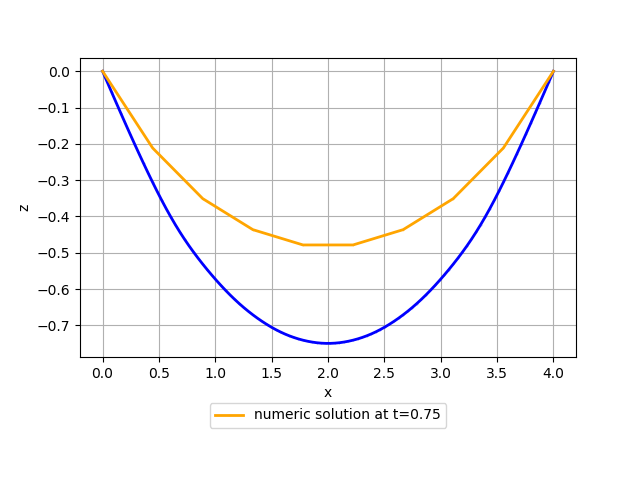
\includegraphics[width=0.7\pagewidth]{plots/075_10_10}
	\caption{График численного и аналитического решений при параметрах $K=10, I=10, t = 0.75с$}
		 \end{center}
	\label{some_pic}
\end{figure}

 \begin{figure}[H]
   \begin{center}
			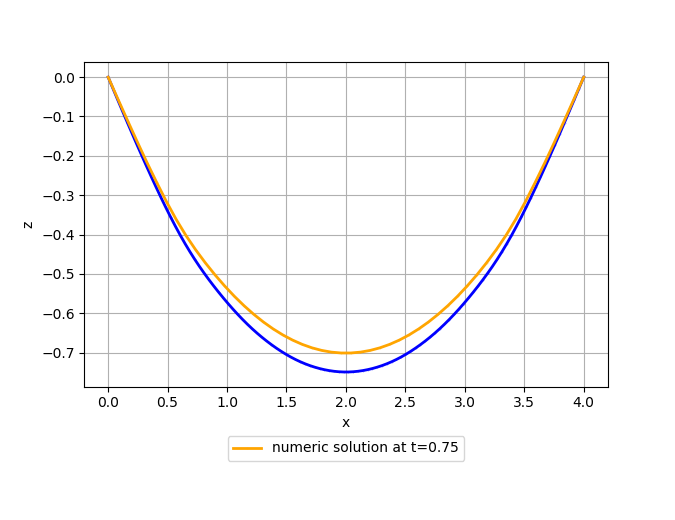
\includegraphics[width=0.7\pagewidth, height=0.4\pageheight]{plots/075_50_50}
	\caption{ График численного и аналитического решений при параметрах $K=50, I=50, t = 0.75с$}
	 \end{center}
	\label{some_pic}
\end{figure}

\begin{figure}[H]
\begin{center}
			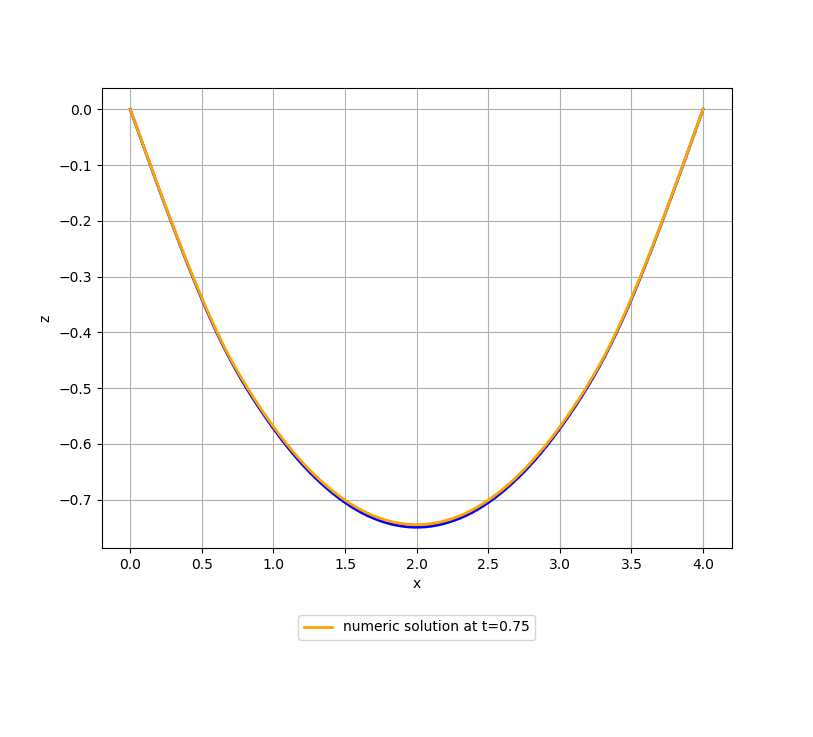
\includegraphics[width=0.7\pagewidth, height=0.4\pageheight]{plots/075_100_100}
	\caption{График численного и аналитического решений при параметрах $K=500, I=500, t = 0.75с$}
	 \end{center}
	\label{some_pic}
\end{figure}

%На рисунках 4-6 приведены графики зависимости концентрации раствора от пространственной переменной $x$ в момент времени $t = 70с$, полученные с помощью схемы Кранка-Николсона.
%\begin{figure}[H]
%\begin{center}
%			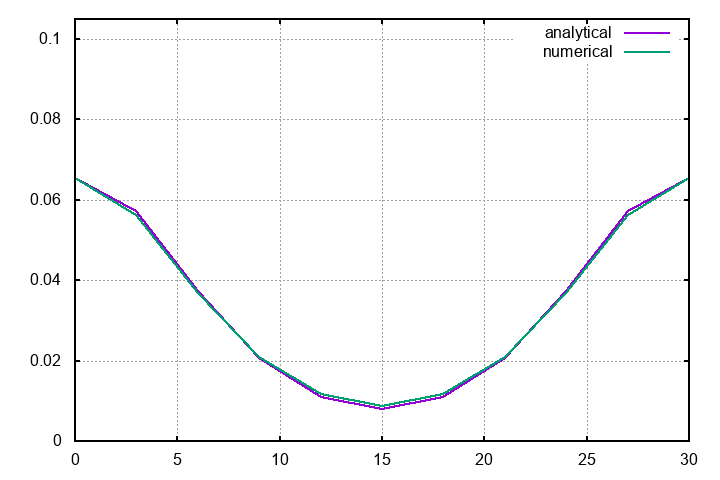
\includegraphics[width=12cm]{plots/kr1}
%	\caption{График численного и аналитического решений при параметрах $K=20, I=10, t = 70с$}
%	 \end{center}
%	\label{some_pic}
%\end{figure}
%
%\begin{figure}[H]
%\begin{center}
%			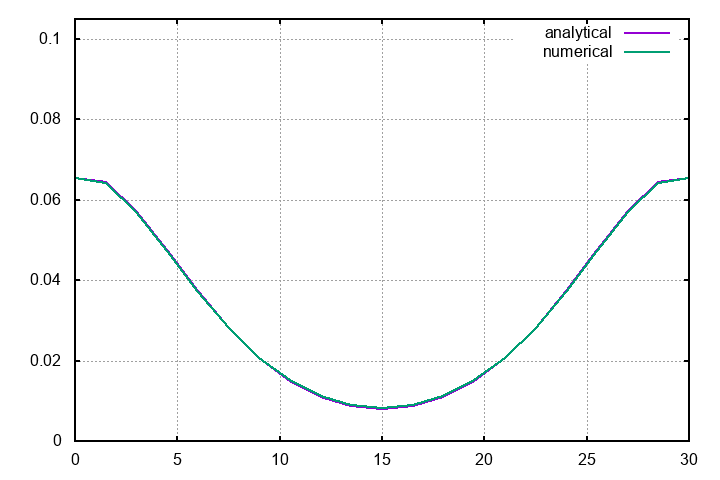
\includegraphics[width=12cm]{plots/kr2}
%	\caption{График численного и аналитического решений при параметрах $K=40, I=20, t = 70с$}
%	 \end{center}
%	\label{some_pic}
%\end{figure}
%
%\begin{figure}[H]
%\begin{center}
%			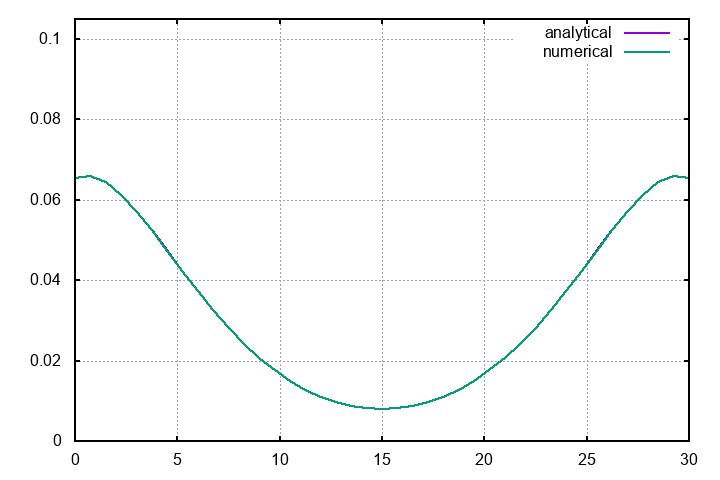
\includegraphics[width=12cm]{plots/kr3}
%	\caption{График численного и аналитического решений при параметрах $K=120, I=40, t = 70с$}
%	 \end{center}
%	\label{some_pic}
%\end{figure}

	Как видно из рисунков 1-3 с увеличением числа узлов сетки наблюдается визуальная сходимость, иными словами численное решение приближается к точному решению исходной задачи.

Исследуем экспериментально скорость сходимости неявной схемы . Для
этого выберем некоторую достаточно крупную сетку и будем ее последовательно
измельчать, каждый раз определяя величину абсолютной погрешности. 

%При этом шаг $h$ будем измельчать в 2 раза, а $\tau$ - в 4 раза. Согласно результатам
%теоретического исследования погрешность сеточного решения для неявной схемы
%характеризуется величиной $O(h^2, \tau)$. Таким образом, следует ожидать, что при
%каждом указанном выше измельчении сетки погрешность численного решения
%будет уменьшаться приблизительно в 4 раза.

%Для неявной схемы погрешность сеточного решения можно описать следующим образом:
%
%\begin{equation}\label{eps}
%	\epsilon_1_{(h, \tau)} = \alpha h^2 + \beta \tau + O(h^3, \tau^2)
%\end{equation}
%\begin{equation}\label{epsby4}
%\epsilon_1_{( \frac{h}{2}, \frac{\tau}{4} )} = \alpha \frac{h^2}{4}  + \beta \frac{\tau}{4}  + O( \frac{h^3}%{8} , \frac{ \tau^2}{16})
%\end{equation}
%		 
%		 Тогда отношение величин \eqref{eps} и \eqref{epsby4} можно оценить следующим образом:	
%		 \begin{equation}\label{eps}
%	\delta_1_{(h, \tau)} = \frac{ \epsilon_1_{ h, \tau } } {\epsilon_1_{ ( \frac{h}{2}, \frac{  \tau }{4})}} %\approx 4
%\end{equation}

Результаты экспериментального исследования сходимости разностной схемы представлены в таблице 1:
		
		\begin{table}[H]
	\centering
	\caption{ Погрешность простейшей явной схемы }
	\begin{tabularx}{0.9\textwidth}{|Y|Y|Y|Y|Y|Y|}
		\hline
		K & I & $h_t$ & $h_x$ & $ \epsilon_{(h, \tau)}$ & $ \delta_{(h, \tau)}$ \\ \hline
		101 & 31 & 1 & 1 & \num{5.04e-4}  & -  \\ \hline
		401 & 61 &  0.25 & 0.5 & \num{1.27e-4} & 3.97  \\ \hline
		1601 & 121 & 0.0625 & 0.25 &   \num{3.17e-5} & 3.99  \\ \hline
\end{tabularx}
	\label{tab1}
\end{table}

%Исследуем экспериментально скорость сходимости схемы Кранка-Николсона . Для
%этого выберем некоторую достаточно крупную сетку и будем ее последовательно
%измельчать, каждый раз определяя величину абсолютной погрешности. При этом
%шаги $h$ и $\tau$ будем измельчать в 2 раза. Согласно результатам
%теоретического исследования погрешность сеточного решения для неявной схемы
%характеризуется величиной $O(h^2, \tau^2)$. Таким образом, следует ожидать, что при
%каждом указанном выше измельчении сетки погрешность численного решения
%будет уменьшаться приблизительно в 4 раза.
%
%Результаты экспериментального исследования сходимости неявной разностной схемы представлены в таблице 2:
%		
%		\begin{table}[H]
%	\centering
%	\caption{ Погрешность схемы Кранка-Николсона }
%	\begin{tabularx}{0.9\textwidth}{|Y|Y|Y|Y|Y|Y|}
%		\hline
%		K & I & $\tau$ & h  & $ \epsilon_{(h, \tau)}$ & $ \delta_{(h, \tau)}$ \\ \hline
%		30 & 10 & 3.33 & 3 & \num{9.07e-04}  & -  \\ \hline
%		60 & 20 &  1.67 & 1.5 & \num{2.36e-04} & 3.84  \\ \hline
%		120 & 40 & 0.83 & 0.75 &   \num{6.01e-05} & 3.93  \\ \hline
%		240 & 80 & 0.42 & 0.38 & \num{1.51e-05} & 3.99 \\ \hline
%\end{tabularx}
%	\label{tab1}
%\end{table}
%
%	Можно заметить, что отношение погрешностей в таблицах 1-2 достаточно близко к ожидаемому теоретическому значению, что убеждает нас в корректной реализации программ для нахождения численного решения задачи диффузии.
		 
		\newpage
	}
	




\titleformat{\section}{\large\bfseries\centering}{\thesection}{0.5em}{\MakeUppercase}
\section*{Заключение}
{
	\addcontentsline{toc}{section}{Заключение}
	В результате выполнения работы осуществлена постановка краевой
задачи для уравнения поперечных колебаний тонкой прямоуголдьной мембраны. Для
численного решения краевой задачи построена простейшая явная разностная схема.

Проведено теоретическое исследование разностной схемы, в результате
которого установлено, что явная схема имеет линейный
порядок аппроксимации для временной переменной и квадратичный для
пространственной переменной.

%С помощью вычислительных экспериментов было показано
 
В результате серии вычислительных экспериментов заметна визуальная
сходимость разностного решения, вычисляемого с помощью схем, при
увеличении количества шагов, т.е. с измельчением сетки решение дискретной
задачи приближается к решению исходной задачи.
}

\newpage

%------------------------------------------------
% Список литературы
%------------------------------------------------
\section*{Список использованных источников}
{
\addcontentsline{toc}{section}{Список использованных источников}
	\begin{enumerate}[label=\arabic*\ \ ]
	\item {Дегтярев А.А. Примеры построения и исследования разностных схем. – Электронное учебное пособие [Электронный ресурс] / А.А Дегтярев, 2011.- 54с.}
	\item {Тихонов А.Н., Самарский А.А. Уравнения математической физики (5-е изд.) [Текст] / Тихонов А.Н., Самарский А.А. М.: Наука, 1977.- 742 с.}
	
	\item {Numpy and Scipy Documentation [Электронный ресурс]: Официальный сайт документации библиотек Numpy и Scipy. - URL: https://docs.scipy.org/doc/}
	
	\item {Свешников А. Г., Боголюбов А. Н., Кравцов В. В. Лекции по математической физике [Текст] / Свешников А. Г., Боголюбов А. Н., Кравцов В. В.  М.:  МГУ, 1993. - 352 с. }
	\end{enumerate}
}
\newpage

%------------------------------------------------
% Приложения. Коды программ и.т.д.
%------------------------------------------------

\section*{Приложение А}
{
	\addcontentsline{toc}{section}{Приложение А Код программы}
	\begin{center}
	\textbf{Код программы}
	\end{center}

	%	\lstinputlisting[language=python,mathescape=false]{sources/main.py}
	\newpage
}

\end{document}
